%%%%%%%%%%%%%%%%%%%%%%%%%%%%%%%%%%%%%%%%%%%%%%%%%%%%%%%%%%%%%%%%%%%%%%%%%%
% File: Lecture_1.tex
% Authors: James Kress
% Date: February 1, 2014
% Description: 
%%%%%%%%%%%%%%%%%%%%%%%%%%%%%%%%%%%%%%%%%%%%%%%%%%%%%%%%%%%%%%%%%%%%%%%%%%

%<<<<<<<<<<<<<<<<<<<<<<<<<<<<<<<<<<<<<<<<<<<<<<<<<<<<<<<<<<<<<<<<<<<<<<<<<<<<<%
% Document package information
%>>>>>>>>>>>>>>>>>>>>>>>>>>>>>>>>>>>>>>>>>>>>>>>>>>>>>>>>>>>>>>>>>>>>>>>>>>>>>%
\documentclass[xcolor=dvipsnames]{beamer} 
%%%%%%%%%%%%%%%%%%%%%%%%%%%%%%%%%%%%%%%%%%%%%%%%%%%%%%%%%%%%%%%%%%%%%%%%%%
% File: _TeXdefs.tex
% Author: James Kress
% Date: January 25, 2014
% Description: A tex file containing the \usepackage declarations, and
%			   other document critial style settings.
%%%%%%%%%%%%%%%%%%%%%%%%%%%%%%%%%%%%%%%%%%%%%%%%%%%%%%%%%%%%%%%%%%%%%%%%%%

%-----------Package imports
\usepackage{graphicx}
\usepackage{pgfpages}
\usepackage{tikz}
\usepackage{latexsym}
\usepackage{verbatim}
%//////////END package imports


%----------Style elements
\useoutertheme{infolines} 
\usetheme{Frankfurt} 
\usepackage{../theme/beamercolorthemeoregon}
\setbeamertemplate{sections/subsections in toc}[default]
\setbeamertemplate{footline}
{
\leavevmode%
  \hbox{%
  \begin{beamercolorbox}[wd=.3\paperwidth,ht=2.25ex,dp=.75ex,center]{institute in head/foot}%
    \usebeamerfont{institute in head/foot}\insertshortinstitute
  \end{beamercolorbox}%
    \begin{beamercolorbox}[wd=.4\paperwidth,ht=2.25ex,dp=.75ex,center]{title in head/foot}%
      \usebeamerfont{title in head/foot}\insertshorttitle
    \end{beamercolorbox}%
  \begin{beamercolorbox}[wd=.3\paperwidth,ht=2.25ex,dp=.75ex,center]{date in head/foot}%
    \usebeamerfont{date in head/foot}\insertshortdate\hspace*{3em}
    \insertframenumber{} / \inserttotalframenumber\hspace*{1ex}
  \end{beamercolorbox}}%
  \vskip0pt%
}
%/////////END style elements


%---------Command Declarations
\DeclareGraphicsExtensions{.pdf, .jpeg, .png, .jpg}
\graphicspath{ {../images/} }
\newcommand{\className}{\text{CIS 410/510} \\ \text{Parallel Computing}}
\newcommand{\departmentName}{\textit{Department of Computer and 
									Information Science \\ University of Oregon}}
%/////////END command declarations


%---------Setup pdf properties
\hypersetup{
	pdfusetitle=true,
    bookmarks=true,         	% show bookmarks bar?
    unicode=false,          	% non-Latin characters in Acrobat’s bookmarks
    pdftoolbar=true,        	% show Acrobat’s toolbar?
    pdfmenubar=true,        	% show Acrobat’s menu?
    pdffitwindow=false,     	% window fit to page when opened
    pdfstartview={Fit},   		% fits the width of the page to the window    
    pdfauthor={},     % author
    pdfsubject={Parallel Programming},   	% subject of the document
    pdfcreator={},   			% creator of the document
    pdfproducer={}, 			% producer of the document
    pdfkeywords={University of Oregon, parallel programming}, 
    pdfnewwindow=true,      	% links in new window
    colorlinks=true,       		% false: boxed links; true: colored links
    linkcolor=white,          	% color of internal links
    hidelinks,
    citecolor=green,        	% color of links to bibliography
    filecolor=magenta,      	% color of file links
    urlcolor=cyan,           	% color of external links
    linktoc=page,
    pageanchor = true
}
%//////////END setup pdf properties


%END ALL


%<<<<<<<<<<<<<<<<<<<<<<<<<<<<<<<<<<<<<<<<<<<<<<<<<<<<<<<<<<<<<<<<<<<<<<<<<<<<<%
% END Document package information
%>>>>>>>>>>>>>>>>>>>>>>>>>>>>>>>>>>>>>>>>>>>>>>>>>>>>>>>>>>>>>>>>>>>>>>>>>>>>>%

%=============================================================================%
% Begining: Title Page Material
%=============================================================================%
\begin{document}
	\title[Lecture 1]{Lecture 1 title ...}
	\author[]{\className}
	\institute[\className]{\departmentName}
	\date{} 

	\titlegraphic{\centering 
		$\vcenter{\hbox{
\includegraphics[height=.31in,width=2.0in]{oregonLogo}}}$
	}

	\begin{frame}
		\maketitle
	\end{frame}
%-----------------------------------------------------------------------------%
% End: Title Page Material
%-----------------------------------------------------------------------------%


%=============================================================================%
% Section -> Map
%=============================================================================%
\section{Map} 

	\begin{frame} \frametitle{Table of Contents}
		\tableofcontents[currentsection]
	\end{frame} 
	
	
	\subsection{Map subsection}
	
		\begin{frame} \frametitle{title}
	
		\end{frame}
%-----------------------------------------------------------------------------%
% End: Map
%-----------------------------------------------------------------------------%

%=============================================================================%
% Section -> SAXPY Example
%=============================================================================%
\section{SAXPY Example} 

	\begin{frame} \frametitle{Table of Contents}
		%\tableofcontents
		%\tableofcontents[pausesections]
		\tableofcontents[currentsection]
	\end{frame} 
	
	
	\subsection{subsection title...}
	
		\begin{frame} \frametitle{title}
	
		\end{frame}
%-----------------------------------------------------------------------------%
% End: SAXPY Example
%-----------------------------------------------------------------------------%

%=============================================================================%
% Section -> Optimizations 
%=============================================================================%
\section{Optimizations} 

	\begin{frame} \frametitle{Table of Contents}
		%\tableofcontents
		%\tableofcontents[pausesections]
		\tableofcontents[currentsection]
	\end{frame} 
	
	
	\subsection{Sequences of Maps}
	
		\begin{frame} \frametitle{Sequences of Maps}
      \begin{columns}
        \begin{column}{0.48\textwidth}
          \begin{itemize}
            \item
              Often several map operations occur in sequence
              \begin{itemize}
                \item
                  Vector math consists of many small operations such as
                  additions and multiplications applied as maps
              \end{itemize}
            \item
              A na\"\i ve implementation may write each intermediate result to
              memory, wasting memory bandwidth and likely overwhelming the
              cache.
          \end{itemize}
        \end{column}
        \begin{column}{0.48\textwidth}
          \centering
          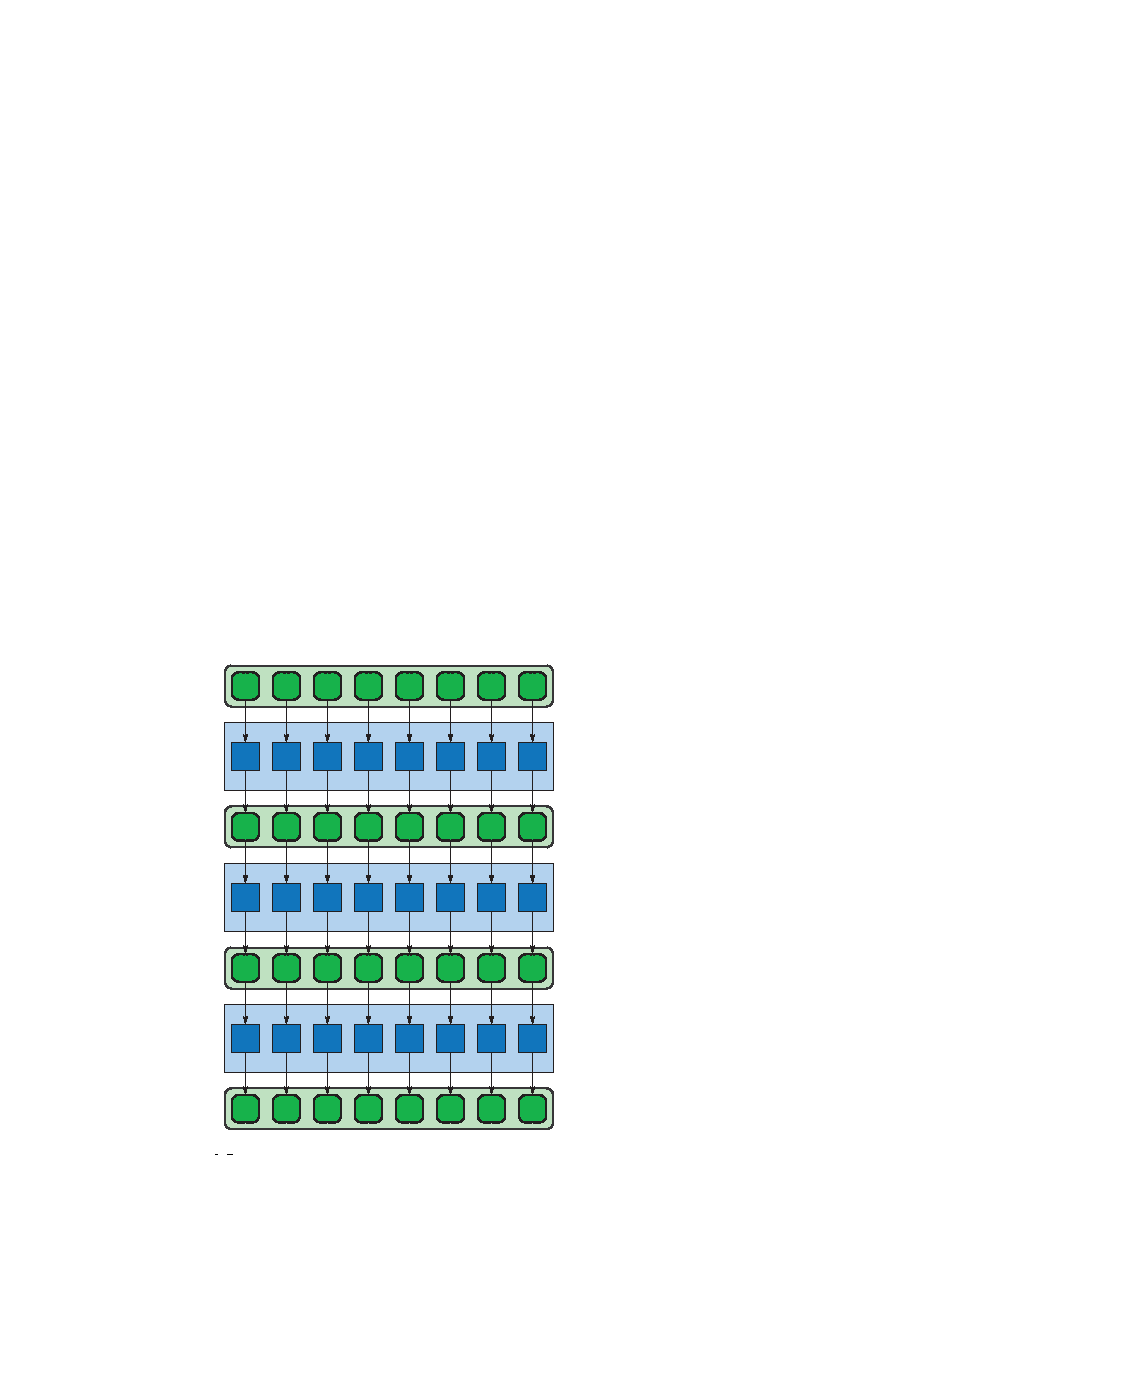
\includegraphics[width=0.9\textwidth]{images/figure-4-2-1}
        \end{column}
      \end{columns}
		\end{frame}

	\subsection{Code Fusion}
		\begin{frame} \frametitle{Code Fusion}
      \begin{columns}
        \begin{column}{0.48\textwidth}
          \begin{itemize}
            \item
              Can sometimes ``fuse'' together the operations to perform them at
              once
            \item
              Adds arithmetic intensity, reduces memory/cache usage
            \item
              Ideally, operations can be performed using registers alone
          \end{itemize}
        \end{column}
        \begin{column}{0.48\textwidth}
          \centering
          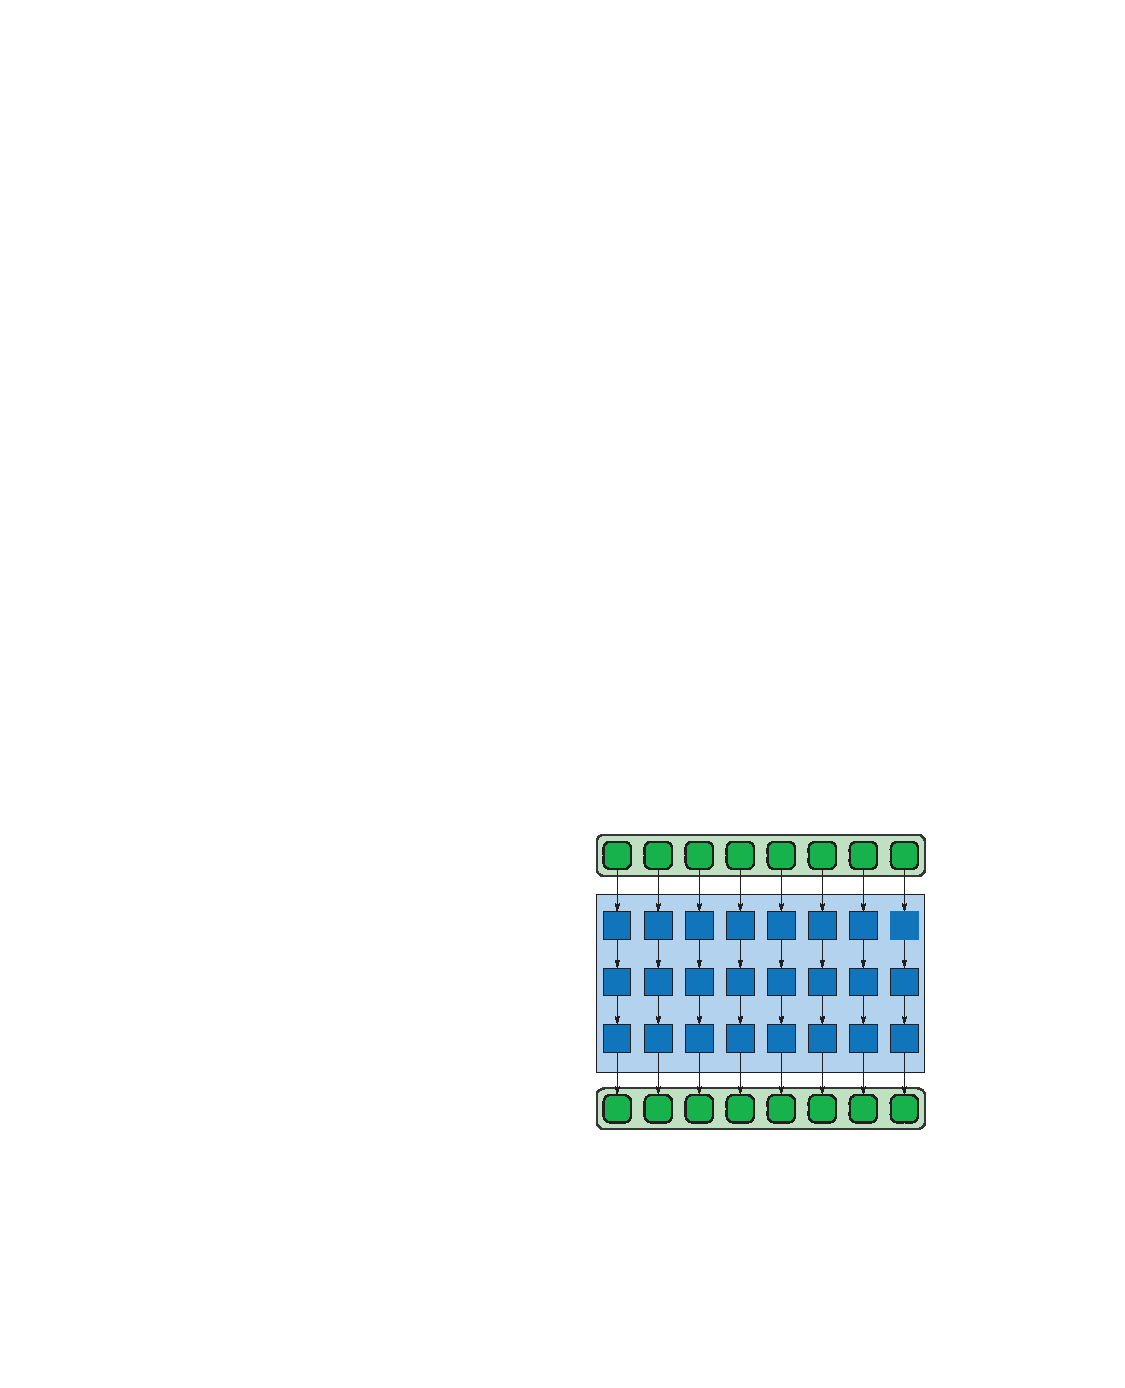
\includegraphics[width=0.9\textwidth]{images/figure-4-2-2}
        \end{column}
      \end{columns}
		\end{frame}

	\subsection{Cache Fusion}
		\begin{frame} \frametitle{Cache Fusion}
      \begin{columns}
        \begin{column}{0.48\textwidth}
          \begin{itemize}
            \item
              Sometimes impractical to fuse together the map operations
            \item
              Can instead break the work into blocks, giving each CPU one block
              at a time
            \item
              Hopefully, operations use cache alone
          \end{itemize}
        \end{column}
        \begin{column}{0.48\textwidth}
          \centering
          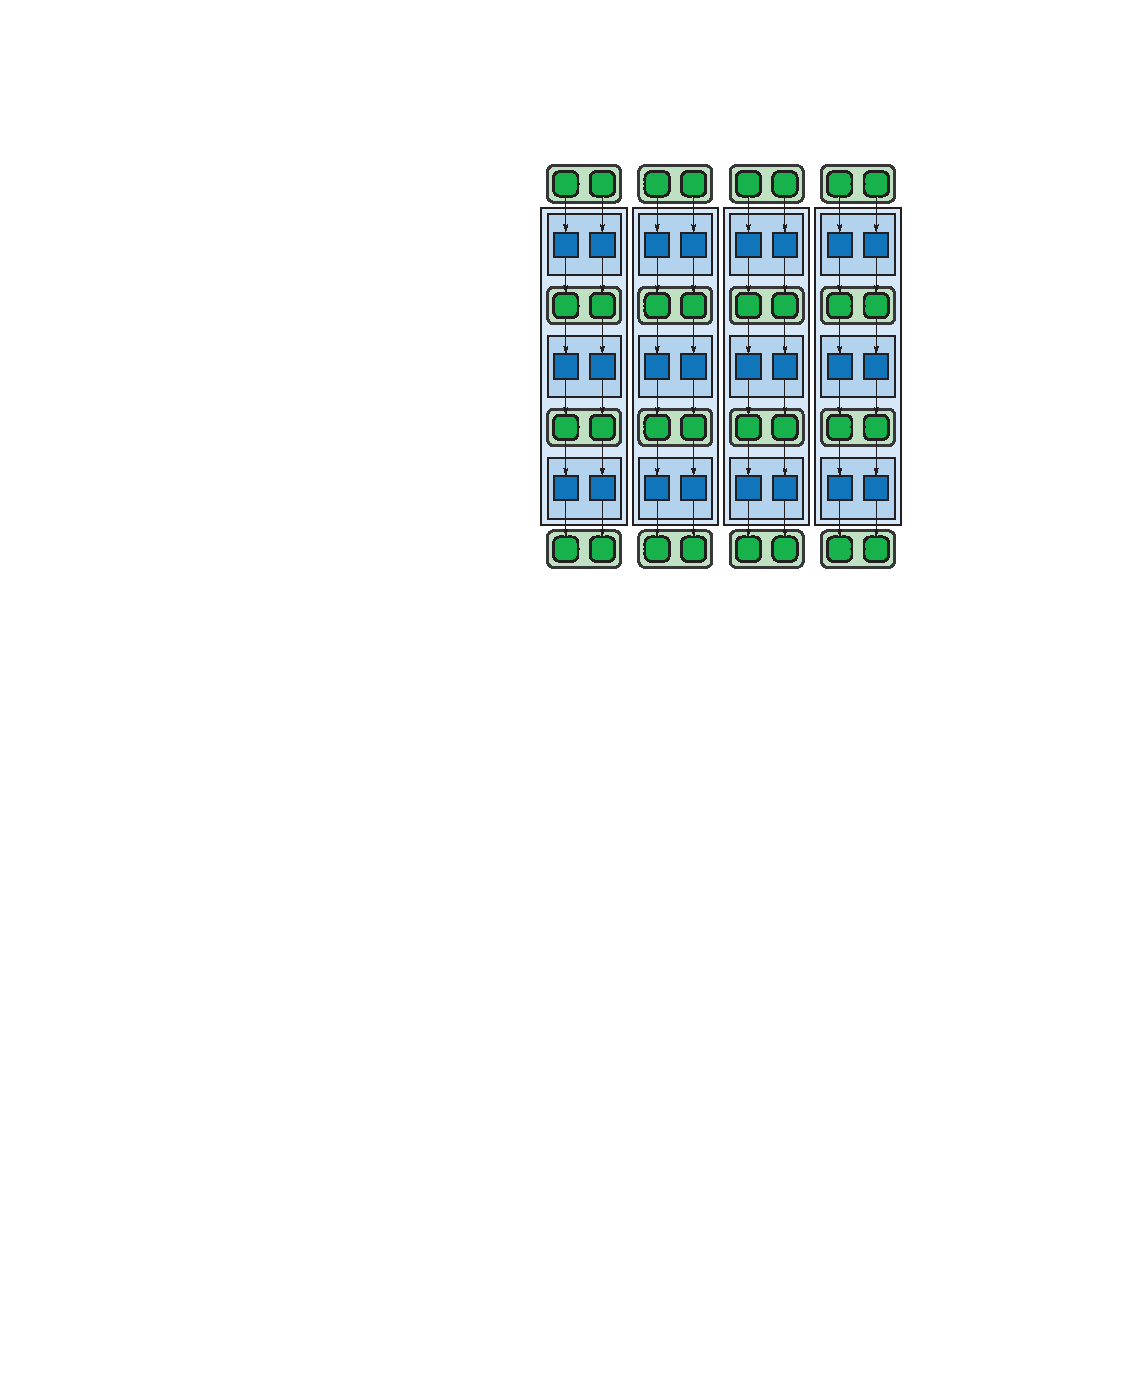
\includegraphics[width=0.9\textwidth]{images/figure-4-3-2}
        \end{column}
      \end{columns}
		\end{frame}
%-----------------------------------------------------------------------------%
% End: Optimizations
%-----------------------------------------------------------------------------%

%=============================================================================%
% Section -> Related Patterns
%=============================================================================%
\section{Related Patterns} 

	\begin{frame} \frametitle{Table of Contents}
		%\tableofcontents
		%\tableofcontents[pausesections]
		\tableofcontents[currentsection]
	\end{frame} 
	
	\subsection{Overview}
	
		\begin{frame} \frametitle{Overview}
			There are several patterns related to map. Three are discussed here: stencil, workpile, and divide-and-conquer. They will be discussed more in detail in a later lecture. Remember maps apply when you can perform the same operation on multiple elements with no dependencies.		
		\end{frame}
	
	\subsection{Stencil}
	
		\begin{frame} \frametitle{Stencil}
			\begin{itemize}
				\item Each instance of the map function accesses neighbors of its input, offset from its usual input
				\item Common in imaging and PDE solvers
			\end{itemize}
		\end{frame}

	\subsection{Workpile}
	
		\begin{frame} \frametitle{Workpile}
			\begin{itemize}
				\item Work items can be added to the map while it is in progress, from inside map function instances
				\item Work grows and is consumed by the map
				\item Workpile pattern terminates when no more work is available
			\end{itemize}
		\end{frame}
		
	\subsection{Divide-and-Conquer}
		
		\begin{frame} \frametitle{Divide-and-Conquer}
			\begin{itemize}
				\item Applies if a problem can be divided into smaller subproblems recursively until a base case is reached that can be solved serially
			\end{itemize}
		\end{frame}
%-----------------------------------------------------------------------------%
% End: Related Patterns
%-----------------------------------------------------------------------------%



\end{document}
%END ALL

